%\begingroup
%\setsecnumdepth{part} 
\chapter{Konklusion} 
\label{chap:konklusion}

Vores mål med dette speciale var, at undersøge muligheden for at lave en udvidelse af \pycsp, der muliggør brugen af tid direkte i sproget. Der findes allerede et massivt teoretisk arbejde indenfor området, men ingen praktisk anvendelige implementeringer, så vores fokus har været på, at det skulle være praktisk anvendeligt. Dette afspejles ved at vi har valgt at benytte eksempler som omdrejningspunkt for vores analyser af de tre anvendelsesområder. 

De tre anvendelsesområder vi identificerede i introduktionen var diskret simulering, realtids-planlægning og interaktiv tid. vi har gennem vores analyse fundet ud af at det er mere hensigtsmæssigt at anskue anvendelsesområderne ud fra hvilken tidsmodel de bygger på. Figur \ref{fig:timemodel} viser således opdelingen af anvendelsesområderne i henholdsvis diskret og real tid.  

\begin{figure}[htp]
 \begin{center}
  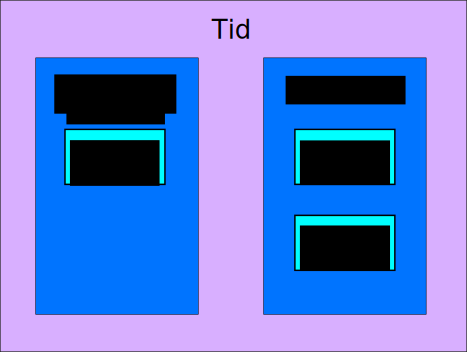
\includegraphics[scale=0.6]{images/timemodel}
	\caption{Forholdet mellem de tre anvendelsesområder af tid vi opstillede i introduktionen.}
	\label{fig:timemodel}
\end{center}
\end{figure}

Indenfor diskret simulering har vi udviklet en løsning, der er let at anvende, og som eliminerer kravet om en delt datastruktur for at administrere tid i \pycsp. Yderligere kræver løsningen væsentligt mindre kode til at administrere tiden, end en tilsvarende løsning lavet i ren \pycsp. 

Sammenligner vi vores løsning med \simpy, der er et framework til simuleringer, skrevet i Python, mener vi at vores løsning er mere intuitiv og fleksibel at benytte, med henblik på at repræsentere arbejdsprocesser der skal simuleres. Dette tillægges i høj grad at vi direkte kan benytte \pycsp's processer. Eksempelvis arbejder \simpy på at udvide deres framework til at kunne håndtere reservation af flere begrænsede ressourser som skal benyttes samtidigt. Dette er allerede muligt i vores løsning, igen grundet at vi bygger på \pycsp, hvorved man kan repræsentere denne reservation ved at lade en proces vente på kommunikation. 

I vores løsning til realtidsplanlægning har vi implementeret EDF, som den grundlæggende algoritme til at bestemme rækkefølgen, for udførsel af processer. Vi har implementeret prioritetsnedarvning for at imødekomme problemer med prioritetsinvertering, og har indført en prioriteret udvælgelse i \code{alternations} og ved kommunikation over kanaler. Vores eksempel viser tydeligt at vores RTP-løsning kan være meget brugtbar, såfremt der i programmet, kan foretages en differentiering i prioriteten af de processer der skal afvikles. 

Vi er kommet frem til at interaktiv planlægning ikke kan anses som et selvstændigt anvendelsesområde, men nærmere som en gren af realtidsplanlægning. De benytte begge reel tid som basis, har deadlines og prioriteter. Interaktiv planlægning har yderligere tilføjet et starttidspunkt, men det ændrer ikke fundamentalt på modellen. 


RTP: estimater for afvikling


Vi har lavet en basisimplementering af RTP der benytter EDF. Det kunne være interessant at kigge på mulighederne for at bedømme en proces' udførselstid, eller lade udvikleren angive dette. Det vil åbne op for brug af andre algoritmer end EDF, hvorved der åbnes op for brug af adskillige andre algoritmer til skemaplanlægningen og udvider anvendelsesområdet.  



%lettere at modellere processer
%Simpy kan ikke reservere begrænsede ressourcer

%Sammenligning med Simpy her 

%Tidsmodeller/anvendelsesområder

%Praktisk anvendelig implementering

%nuværende tilstand for anvendelsesområderne

%\endgroup 

